\documentclass[]{./MFFPrace}

\usepackage[starfontserif]{starfont}
\usepackage{caption}

\NazevPrace{Identifikace meteorických rojů}
\NazevPraceEN{Meteor Shower Identification}
\AutorPrace{Michal~Ciesla}
\RokOdevzdani{2024}
\Katedra{Astronomický ústav AV ČR}
\KatedraEN{Astronomical~Institute, Academy of Sciences of the Czech Republic}
\TypPracoviste{Ústav}
\TypPracovisteEN{Institute}
\Vedouci{RNDr.~Pavel~Koten,~Ph.D.}
\KatedraVedouciho{\IKatedra}
\KatedraVedoucihoEN{\IKatedraEN}
\StudijniProgram{Fyzika}
\StudijniObor{FP\ask{Opravdu jen takto zkratkou?}}
\Podekovani{\todo{Napsat poděkování}}
\Abstrakt{\todo{Napsat abstrakt}}
\AbstraktEN{From observations of meteors, we are able to determine the orbit of the meteoroid. We then decide which meteor shower the observed meteor belongs to based on the orbital elements of this orbit. Several methods, collectively known as $D$-criteria, have been devised for this exact purpose. These are based on an orbital dissimilarity measure the value of which is then compared with some fixed cutoff value. We describe the $D_\text{SH}$, $D_\text{D}$, $D_\text{H}$ and $D_\text{N}$ criteria and discuss their properties. These findings are used to create a software tool which applies these criteria to real-world data.}
\KlicovaSlova{{meteorické roje}, {$D$-kritérium}, {míra orbitální odlišnosti} \todo{Vypsat klíčová slova}}
\KlicovaSlovaEN{{meteor swarms}, {$D$-criterion}, {orbital dissimilarity measure} \todo{Write out keywords}}

\addbibresource{literatura.bib}

\captionsetup{justification=centering}

\begin{document}
    \maketitle
    \tableofcontents
    \begin{todolist}
        \pagebreak
        \item[\done] Úvod
        \item Observace, měření a reprezentace
        \begin{todolist}
            \item[\done] Elementy dráhy
            \item[\done] Fotografická měření
        \end{todolist}
        \item Historické metody klasifikace
        \begin{todolist}
            \item Přímé porovnávání elementů dráhy
            \item Funkce orbitální odlišnosti, $D$-kritérium
        \end{todolist}
        \item Revidované heliocentrické metody
        \begin{todolist}
            \item Revidovaná funkce odlišnosti $D_\text{D}$ a příslušnost kometám
            \item Hybridní funkce $D_\text{H}$
        \end{todolist}
        \item Geocentrický přístup
        \begin{todolist}
            \item Semi-invariantní orbitální veličiny
            \item Geocentrická funkce $D_\text{N}$
        \end{todolist}
        \item Porovnání úspěšnosti metod klasifikace
        \item Praktická část
        \item Závěr
    \end{todolist}
    \noindent
    
    \chapwithtoc{Úvod}% MARK: Úvod

\textit{Meteory} jsou světelné stopy vznikající při průletu menších těles -- \textit{meteoroidů} -- atmosférou Země či jakéhokoliv jiného\footnote{Ačkoli je definice \cite{meteorastro} velmi obecná v tělese, kam meteoroid padá, budeme se zajímat pouze o meteory pozorované v atmosféře Země.} vesmírného tělesa \cite{meteorastro}.\footnote{\textit{Meteorit} je posledním z matoucích termínů v meteorické astronomii, jedná se o pevný zbytek meteoroidu po průletu atmosférou, který dopadne na povrch Země nebo jiného vesmírného tělesa \cite{meteorastro}. Ne všechny meteoroidy zanechávají meteority, některé se mohou v atmosféře úplně odpařit.} Samotné meteory jsou velkolepým úkazem, z astronomického hlediska je však více než jednotlivé meteory zajímavá souvislost mezi nimi: Jelikož meteoroidy vznikají často jako úlomky z komet či planetek \cite{meteorastro}\cite{cometassoc}, ukazuje se, že lze pozorované meteory často zařadit do "`rodin"' zvaných \textit{meteorické roje}.

Meteory můžeme buďto přiřadit do nějakého roje, nebo do tzv. \textit{sporadického pozadí}. \ask{Následuje spekulace. Je nějaké dobré místo, kde o historii zjistit více?} Historicky se meteory pozorovaly hlavně okem, případně s pomocí dalekohledů, a do rojů se zařazovaly podle ročního období (nebo konkrétněji, měsíce) a směru, odkud se jevily přilétat. Příchod a rozvoj obrazových záznamových médií od prvních fotografických emulsí až po současné videozáznamy však umožnil meteory zaznamenávat a detailně studovat jejich vlastnosti. Se zvyšováním dostupnosti fotografických zařízení, vývojem citlivějších záznamových médií a nástupem automatizace významně narostl počet pozorovacích stanic po celé Zemi a tím pádem ohromný nárůst spatřených a zaznamenaných meteorů.

Tento velký objem pozorovaných meteorů společně s potřebou zpřesňování měření a klasifikace pro další vývoj astronomie vedl ke snaze provádět zařazování jednotlivých meteorů do meteorických rojů (či do sporadického pozadí) rigorózními způsoby založenými hlavně na dráze meteoroidu \cite{dsh} v meziplanetárním prostoru -- jelikož jsou meteoroidy často úlomky z jistého mateřského tělesa \cite{meteorastro}\cite{cometassoc}, dá se předpokládat, že úlomky ze stejného tělesa budou mít podobné dráhy \cite{dsh}.

Většina používaných metod zařazování meteorů staví na metodě Southwortha a Hawkinse \cite{dsh}, která je založená na výpočtu míry "`orbitální odlišnosti"' z elementů dráhy meteoroidů. Těmito metodami se budeme dále zabývat, nicméně je vhodné zmínit, že s nástupem informačních technologií a strojového učení ("`machine-learning"') se nepochybně objevily i metody založené právě na strojovém učení. Jelikož ale strojové učení funguje v principu do velké míry jako "`černá skříňka,"' není prakticky příliš možné popisovat vlastnosti či fyzikální pozadí těchto metod.
    \chapter{Observace, měření a reprezentace}
K pozorování meteorů a jejich záznamu se v současnosti používají tři přístupy: fotografické snímky, videozáznamy a radarová měření.

Ve všech třech přístupech je cílem sledovat a zaznamenávat celou oblohu nebo alespoň její velkou část. Například u fotografického přístupu se používá rybí oko \cite{ceplecha} -- čočka nebo objektiv, který je schopný zobrazit celou oblohu na jeden snímek. Cenou za takto širokoúhlý snímek je velké zkreslení obrazu, to lze ale pro účely měření matematicky odstranit \cite{ceplecha}.

\todo{Radarová měření dle \cite{radiosurvey}}

Fotografické snímky a videozáznamy jsou z hlediska měření velmi blízké: Videozáznam je v principu pouze série fotografií, v minulém století se ale využívalo spíše opačného přístupu, kdy se několik fotografických záběrů zaznamenalo na jeden snímek \cite{ceplecha}. Oba přístupy tedy dávají průběh polohy (a případně i luminosity) meteoru v čase. Konkrétně pro metody identifikace meteorických rojů potřebujeme právě dráhu (polohu) a rychlost meteoru \cite{ceplecha}, abychom zjistili orbitální dráhu meteoroidu. Důkladněji se zpracování fotografických snímků budeme věnovat v sekci \ref{sec:foto}.

\section{Elementy dráhy}
Orbitální dráhy jsou v prvním přiblížení elipsy, které jsou nakloněné v prostoru. Jedním z ohniskových bodů je vždy těžiště (Sluneční) soustavy, pro určení dráhy tedy stačí 5 parametrů \cite{astro}.

\medskip

Dva z parametrů popisují tvar elispy; její velikost a excentricitu \cite{astro}. \textit{Excentricita} $e$ náleží do intervalu $\left[0,1\right)$,\footnote{Excentricita může být také $=1$ pro parabolické a $>1$ pro hyperbolické dráhy. \ask{Otevřené, předpokládám, ignorujeme, protože by patřily do sporadického pozadí automaticky (nemají mateřský objekt ve Sluneční soustavě).}} a udává, jak blízká kružnici tato dráha je (viz obrázek \ref{img:excentricity}).

\todo{Ilustrace excentricit}

Pro určení velikosti používáme buďto \textit{délku hlavní poloosy} $a$ nebo \textit{vzdálenost perihelia} $q$ (efektivně vzdálenost okraje elipsy od ohniska). Jejich vztah ilustruje obrázek \ref{img:elipsa} a mezi oběma lze převádět pomocí rovnice \cite{ceplecha}
$$
    q=a(1-e)\text{.}
$$

\todo{Obrázek vztahu mezi $a$ a $q$}

\smallskip

Zbylé tři parametry určují natočení elipsy v prostoru. Jedná se o obdobu Eulerových úhlů, jsou ovšem definované vůči Slunci a ekliptice. Tyto úhly jsou znázorněny v obrázku \ref{img:elementy} a slovně se jedná o
\begin{itemize}
    \item \textit{inklinaci} $i$, která udává úhel mezi rovinou ekliptiky a rovinou elipsy \cite{astro},
    \item \textit{délku vzestupného uzlu} $\Omega$, která udává heliocentrickou ekliptikální délku bodu, ve kterém dráha protíná rovinu ekliptiky při průletu z jihu (tzv. \textit{vzestupný uzel}, \NorthNode) \cite{astro}, a
    \item \textit{argument perihelia} $\omega$, úhel, ve kterém se nachází perihelium, měřený od úsečky spojující Slunce a vzestupný uzel \cite{astro}.
\end{itemize}
Tyto úhly se aplikují jako rotace na rovinu ekliptiky s počátkem ve středu Slunce.

\begin{figure}[ht]
    \centering
    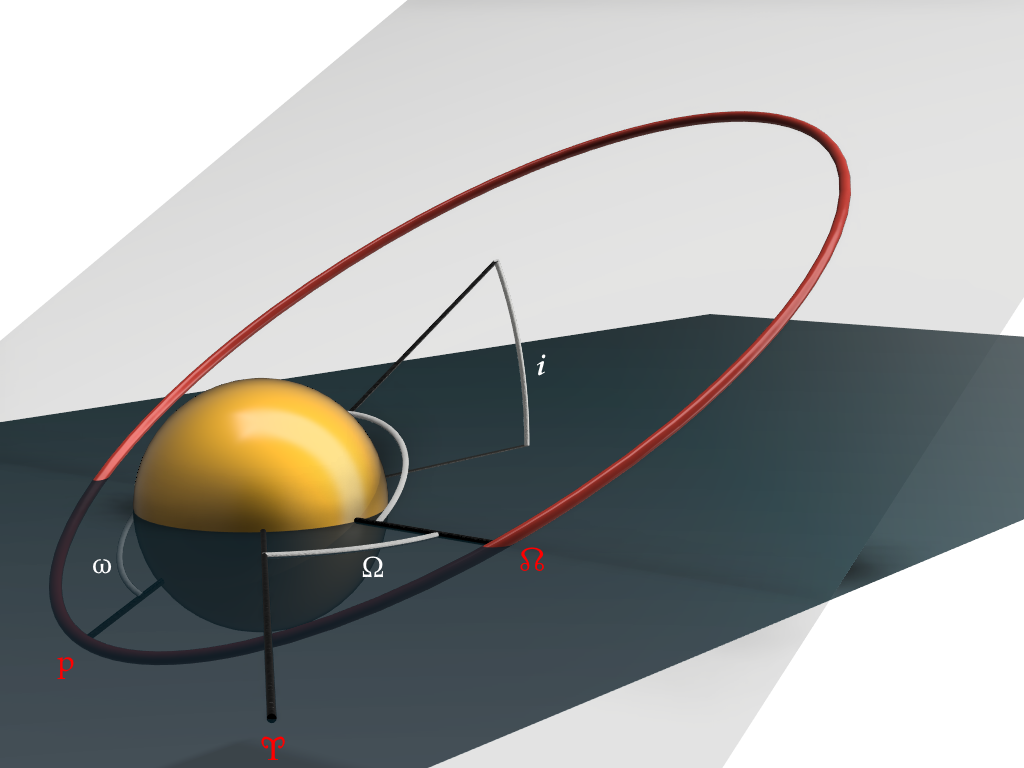
\includegraphics[width=0.8\linewidth]{img/orbit-elements-marked.png}
    \caption{Ilustrace významu elementů dráhy $i$, $\Omega$ a $\omega$ \cite{astro}}
    \label{img:elementy}
\end{figure}

\medskip

Na takto definované dráze se ještě můžeme setkat se souřadnicí zvanou \textit{pravá anomálie} $\nu$. Ta již nespecifikuje dráhu, nýbrž polohu objektu na své dráze, a v meteodách identifikace meteorických rojů nevystupuje. Udává se jako úhel měřený od spojnice Slunce a perihelia ke spojnici Slunce a objektu \cite{astro}.

\section{Fotografická měření\label{sec:foto}}
Úkolem astrometrických měření meteorů je zjistit elementy dráhy meteoroidu před tím, než se setkal s atmosférou Země. Vše ale začíná na fotografii nebo videozáznamu průletu meteoru atmosférou.

Budeme popisovat techniku měření používanou pro fotografická měření, kde máme fotoaparát s rybím okem pro zachycení celé oblohy a clonou, která s pevnou periodou (několikrát za vteřinu) zakrývá detektor nebo fotografický film, čímž zachytí časovou závislost pohybu meteoru. \todo{Bude-li obrázek, přidat a popsat.} Pro video je postup prakticky identický, hůře se ale ilustruje.

\medskip

Mějme tedy stanici \textbf{A} ležící na zeměpisné šířce $\varphi_\mathbf{A}$ a zeměpisné délce $\lambda_\mathbf{A}$, kde je umístěn fotoaparát s rybím okem a periodickou clonou tak, že zenit (kolmice k zemskému geoidu) leží uprostřed snímku, a přesné hodiny pro zaznamenání času měření. Fotoaparát v průběhu noci pořídí velké množství snímků a ke každému snímku umíme přiřadit přesný čas. Stejně tak mějme dále stanici \textbf{B}.

\note{Přidat vysvětlení, proč se pracuje s protínáním rovin, a ne prostě triangulací polohy.}

\smallskip

%#region Kroky (1)-(3): Měření kartézských souřadnic, převod na obzorníkové souřadnice, převod na rovníkové souřadnice II. druhu
Prvním krokem při zachycení meteoru je získat z fotografie jeho polohu v obzorníkové soustavě. K tomu nejprve snímek zkalibrujeme.

Začneme zavedením kartézských souřadnic na snímku s počátkem ve středu fotografie, který by měl být polohou zenitu. Přepočet z kartézských souřadnic $x,\,y$ na obzorníkové souřadnice $A,\,z$ provedeme pomocí vzorců \cite{ceplecha}
\begin{eqnarray}
    \begin{aligned}
        \tan{A-A_0}&=\frac{y-y_0}{x-x_0}\\
        z&=U+V\cdot r+S\cdot e^{D\cdot r}\text{, kde}
    \end{aligned}\label{eqn:lsqr}\\
    r^2=(x-x_0)^2+(y-y_0)^2\text{.}
\end{eqnarray}
Ve vzorcích \eqref{eqn:lsqr} jsou proměnné $A_0,\,x_0,\,y_0,\,U,\,V,\,S$ a $D$ neznámé a jejich hodnoty zjistíme fitováním metodou nejmenších čtverců z poloh hvězd.

Na snímku identifikujeme hvězdy, z katalogu zjistíme jejich polohy a pomocí geografické polohy a času měření přepočteme polohy hvězd do obzorníkových souřadnic $A_{\ast i},\,z_{\ast i}$. Na snímku také odměříme kartézkské souřadnice těchto hvězd $x_{\ast i},\,y_{\ast i}$. Páry souřadnic poté použijeme pro zjištění neznámých proměnných metodou nejmenších čtverců (detailně viz \cite[223--224]{ceplecha}).

S kompletními převodními vztahy \eqref{eqn:lsqr} převedeme jednotlivé otisky meteoru na jednom snímku z odměřených kartézských poloh $x_i,\,y_i$ na obzorníkové $A_i,\,z_i$. Ty následně přepočteme do rovníkových souřadnic {\uppercase\expandafter{\romannumeral 2\relax}}. druhu; za použití času měření $\vartheta_i$ a geografické polohy stanice $\varphi_\mathbf{A},\,\lambda_\mathbf{A}$ získáme deklinaci $\delta_i$ a rektascenzi $\alpha_i$ \cite{ceplecha}.
%#endregion

\smallskip

%#region Kroky (4)-(7): Nalezení střední roviny otisků ze stanice A
Z jednotlivých souřadnic $\delta_i,\,\alpha_i$ zadefinujeme složky
\begin{equation}
    \begin{aligned}
        \xi_i&=\cos{\delta_i}\cos{\alpha_i}\\
        \eta_i&=\cos{\delta_i}\sin{\alpha_i}\\
        \zeta_i&=\sin{\delta_i}
    \end{aligned}
\end{equation}
jednotkových vektorů
$$
\vec{\rho}_i=\begin{pmatrix}
    \xi_i\\\eta_i\\\zeta_i
\end{pmatrix}\text{,}
$$
které ukazují do směru jednotlivých otisků meteoru relativně vůči poloze stanice. V ideálním případě by všechny vektory $\left\{\vec{\rho}_i\right\}$ ležely v rovině, při reálných měřeních se ale od jisté střední roviny mírně odchylují. Zavedeme tedy (jednotkový) vektor $\vec{n}_\mathbf{A}$ jako normálový vektor definující tuto střední rovinu podmínkou, aby byl co nejvíce kolmý na $\vec{\rho}_i$, resp. přesněji jako jednotkový vektor $\vec{m}\in S_3(1)$ takový, že suma
$$
    \sum_{i}{\left( \vec{m}\cdot\vec{\rho_i} \right)^2}
$$
je minimální \cite{ceplecha} (suma by byla rovna nule, pokud by vektory $\vec{\rho}_i$ ležely v rovině).

Pro tuto podmínku lze analyticky nalézt jednoznačné řešení, kterým je \cite{ceplecha}
\begin{equation}
    \begin{aligned}
        \vec{n}^\prime=\begin{pmatrix}
            \left( \sum_{i}{\xi_i\eta_i} \right)\left( \sum_{i}{\eta_i\zeta_i} \right)-\left( \sum_{i}{\eta_i^2} \right)\left( \sum_{i}{\xi_i\zeta_i} \right)\\
            \left( \sum_{i}{\xi_i\eta_i} \right)\left( \sum_{i}{\xi_i\zeta_i} \right)-\left( \sum_{i}{\xi_i^2} \right)\left( \sum_{i}{\eta_i\zeta_i} \right)\\
            \left( \sum_{i}{\xi_i^2} \right)\left( \sum_{i}{\eta_i^2} \right)-\left( \sum_{i}{\xi_i\eta_i} \right)^2
        \end{pmatrix}\text{.}
    \end{aligned}
\end{equation}
Normalizací pak získáme požadovaný jednotkový vektor
\begin{equation}
    \vec{n}_\mathbf{A}=\frac{\vec{n}^\prime}{\lVert \vec{n}^\prime \rVert }\text{.}
\end{equation}

\smallskip

K určení roviny potřebujeme kromě normálového vektoru také jeden bod, kterým je v našem případě pozorovací stanice. Její geografické souřadnice známe, potřebujeme ale přejít do souřadinic geocentrických, ve kterých budeme provádět dalších několik kroků.

Geocentrické souřadnice udávají vzorce \cite{ceplecha}
\begin{equation}
    \begin{aligned}
        X&=(R+h)\cos{\varphi^\prime}\cos{\vartheta}\\
        Y&=(R+h)\cos{\varphi^\prime}\sin{\vartheta}\\
        Z&=(R+h)\sin{\varphi^\prime}\text{,}
    \end{aligned}
    \label{eqn:geocentric}
\end{equation}
kde $h$ je nadmořská výška objektu, $\vartheta$ je místní hvězný čas, $R$ je poloměr Země v kilometrech korigovaný na tvar geoidu v zeměpisné šířce $\varphi$ daný vzorcem \cite{ceplecha}
\begin{equation}
    R=\sqrt{40\,680\,669{,}86\frac{1-0{,}013\,343\,955\,4 \sin^2{\varphi}}{1-0{,}006\,694\,385\,096 \sin^2{\varphi}}}
\end{equation}
a $\varphi^\prime$ je geocentrická zeměpisná šířka \cite{ceplecha}
\begin{equation}
    \begin{aligned}
        \varphi^\prime=\varphi&-0{,}192\,424\,086\,7^\circ \sin{2\varphi}\;+\\
        &+0{,}000\,323\,122^\circ \sin{4\varphi}\;-\\
        &-0{,}000\,000\,723\,5^\circ \sin{6\varphi}\text{.}
    \end{aligned}
\end{equation}

Provedeme-li skalární součin normálového vektoru $\vec{n}_\mathbf{A}$ s vektorem geocentrické polohy stanice $\vec{a}=\left(\begin{smallmatrix}
    X\\Y\\Z
\end{smallmatrix}\right)$, získáme vzdálenost
\begin{equation}
    d_\mathbf{A}=\vec{n}_\mathbf{A}\cdot\vec{a}
\end{equation}
roviny od středu Země \cite{ceplecha} a rovinu pak můžeme zapsat rovnicí \cite{ceplecha}
\begin{equation}
    \vec{n}_\mathbf{A}\cdot\vec{\rho}=d_\mathbf{A}\text{.}
    \label{eqn:photo:plane_a}
\end{equation}
%#endregion

\medskip

%#region Kroky (8)-(12): Protnutí rovin pro přesnou lokalizaci otisku, získat polární souřadnice
Stejný postup zopakujeme pro stanici \textbf{B} s geocentrickým polohovým vektorem $\vec{b}$, kde na konci získáme druhou rovinu s rovnicí
\begin{equation}
    \vec{n}_\mathbf{B}\cdot \vec{\rho}=d_\mathbf{B}\text{.}
    \label{eqn:photo:plane_b}
\end{equation}
Průsečnice těchto dvou rovin je přímka, po které uvažujeme, že se meteor skutečně pohyboval -- jakási střední trajektorie, s jejíž pomocí odstraňujeme nepřesnosti záznamového média a technik přepočtu. Tato přímka je navíc určená i se vzdáleností od středu Země podle vzorců \eqref{eqn:geocentric}, kterou jsme doposud neznali.

\smallskip

Geocentrickou polohu jednotlivých otisků meteoru zjistíme s pomocí ještě třetí roviny, kterou zavedeme pro každý otisk meteoru: Pro jednu z pozorovacích stanic, uvažujme například stanici \textbf{A}, definujeme rovinu takovou, že obsahuje polopřímku tvořenou stanicí \textbf{A} s polohovým vektorem $\vec{a}$ a vektorem $\vec{\rho}_i$ a je kolmá na rovinu definovanou normálovým vektorem $\vec{n}_\mathbf{A}$ (rovnicí \eqref{eqn:photo:plane_a}). Tuto rovinu můžeme opět reprezentovat normálovým vektorem \cite{ceplecha}
\begin{equation}
    \vec{n}_i=\vec{\rho}_i\times\vec{n}_\mathbf{A}
\end{equation}
a vzdáleností
\begin{equation}
    d_i=\vec{n}_i\cdot \vec{a}\text{.}
\end{equation}
Tuto rovinu také můžeme zapsat ve tvaru rovnice a protnutím této roviny s rovinami \eqref{eqn:photo:plane_a} a \eqref{eqn:photo:plane_b} nalezneme polohu otisku meteoru na jeho střední trajektorii \cite{ceplecha}:
\begin{equation}
    \tag{\ref{eqn:photo:plane_a}}
    \vec{n}_\mathbf{A}\cdot\vec{\rho}=d_\mathbf{A}
\end{equation}
\begin{equation}
    \tag{\ref{eqn:photo:plane_b}}
    \vec{n}_\mathbf{B}\cdot\vec{\rho}=d_\mathbf{B}
\end{equation}
\begin{equation}
    \vec{n}_i\cdot\vec{\rho}=d_i
\end{equation}

Vyřešením této soustavy rovnic získáme jednoznačně určený vektor $\vec{\rho}$, který si pro účely dalších výpočtů přeznačíme na $\vec{\rho}\equiv\vec{r}_i$. Vektor $\vec{r}_i$ již není jednotkovým vektorem, nýbrž udává geocentrickou polohu meteoru v bodě $i$-tého otisku. Z jeho složek dostaneme pomocí vzorců \eqref{eqn:geocentric} zpět polární souřadnice; geocentrickou šířku $\varphi^\prime_i$, hodinový úhel $\vartheta_i$ a vzdálenost $(R+h_i)=\lVert\vec{r}_i\rVert$.
%#endregion
    \chapter{Historické metody klasifikace}% MARK: Historické metody klasifikace
Nejjednodušší a také historicky používanou metodou klasifikace meteorických rojů bylo pouhé porovnání polohy radiantu (bodu na nebeské sféře, odkud meteory jednoho roje zjevně přilétají \cite{glossary}) a geocentrické rychlosti \cite{radiosurvey}. Z této metody také vychází způsob pojmenování meteorických rojů: Roje dostávají jméno podle hvězdy, která je na nebi nejblíže radiantu \cite{dsh}. Získáváme tak názvy jako např. \textit{Perseidy}, \textit{Jižní $\delta$ Aquaridy} nebo \textit{Severní Tauridy}.

Bylo ale rozhodnuto, že pro prvotní klasifikaci meteorických rojů budou používány elementy dráhy, které lépe vystihují původ meteoroidů a nemění se v čase tak rychle jako polohy radiantů \cite{radiosurvey}.

\medskip

Všechna následující kritéria pracují na jednoduchém principu: Vezmeme elementy dráhy dvou meteoroidů a pomocí daného kritéria ověříme, zda patří do stejného roje či nikoliv. Máme-li meteoroidů více, po dvojicích ověřujeme kritérium a sestavujeme tak třídy ekvivalence meteoroidů -- kandidáty na meteorické roje. Obdobně, máme-li je k dispozici, můžeme využít střední elementy dráhy známých meteorických rojů a nově pozorovaný meteor zkusit přiřadit do některého z nich.

Pokud třída ekvivalence má dostatek prvků (více než 2 meteoroidy \cite{radiosurvey}), jedná se pravděpodobně o meteorický roj. Podle četnosti se meteorické roje dále děli na hlavní a vedlejší. Pokud však meteoroid tvoří třídu ekvivalence jen sám nebo jen s několika málo dalšími meteoroidy, zařazujeme jej do \textit{sporadického pozadí}, tedy meteoroidů, které se oddělily samostatně, jsou již staré a byly příliš perturbovány pohybem planet \cite{dsh}, nebo nepocházejí ze Sluneční soustavy.

\section{Přímé porovnávání elementů dráhy}% MARK: Přímé porovnání elementů dráhy
\citeauthor{radiosurvey} nebyl prvním, kdo přišel s úspěšným kritériem přiřazování meteorů do meteorických rojů, ale v \cite{radiosurvey} publikoval jednoduše uchopitelné a efektivní kritérium: Zda se elementy dráhy dvou meteoroidů liší o méně než jisté stanovené hodnoty.

Kritérium zavedené \citeauthor{radiosurvey}em bere pro dva meteoroidy elementy dráhy $a_i$, $e_i$, $i_i$ a $\nu_i$ a říká, že tyto dva meteoroidy spadají do stejného roje, pakliže splňují všechny následující podmínky \cite{radiosurvey}:
\begin{eqnarray}
    \left|\frac{1}{a_1}-\frac{1}{a_2}\right| &\le& 0{,}15 \text{,}\\
    \left|e_1-e_2\right| &\le& 0{,}07 \text{,}\\
    \left|i_1-i_2\right| &\le& 7^\circ \text{,}\\
    \left|\nu_1-\nu_2\right| &\le& 7^\circ \label{eqn:history:anomaly}\text{.}
\end{eqnarray}
Poslední podmínka je ještě doplněna o případ, kdy je excentricita alespoň jednoho meteoroidu malá: $e<0{,}3$ \cite{radiosurvey}. Mění se pak na \cite{radiosurvey}
\begin{equation}
    \tag{\ref{eqn:history:anomaly}*}
    \left|\nu_1-\nu_2\right| \le 7^\circ+100(0{,}3^\circ-e)\text{.}
\end{equation}
\citeauthor{radiosurvey} ale dodává, že v praxi se toto upřesnění neuplatní, jelikož nebyly známy žádné meteorické roje s $e<0{,}4$ \cite{radiosurvey}. Dále by se žádné dva meteoroidy z daného meteorického roje neměly lišit o více než dvojnásobek limitu \cite{radiosurvey}.

\section{Míra orbitální odlišnosti, $D$-kritérium}% MARK: Míra orbitální odlišnosti, D-kritérium
% \cite{dsh} \cite[220]{radiosurvey} \cite[604]{remarks} \cite{newapproach} \cite[623]{galligan}
\citeauthor{dsh} navrhli koncept číselné míry orbitální odlišnosti dvou meteoroidů: Zavedli funkci $D(A,B)$, jejíž hodnota je mírou odlišnosti orbitů meteoroidů $A$ a $B$, a obdobně funkci $D(M,N)$, která má stejný matematický předpis, ale porovnává dráhu meteoroidu $N$ se střední dráhou známého roje $M$ \cite{dsh}. S jejich pomocí předložili tři možné metody klasifikace:
\begin{enumerate}
    \item Funkci $D(A,B)$ aplikujeme na všechny dvojice meteoroidů a ověřujeme, zda je její hodnota menší než jistá hraniční hodnota $D_S$ \cite{dsh}. Tvoříme tak třídy ekvivalence (podobně jako v \citeauthor{radiosurvey}ově metodě) a roj identifikujeme jako třídu ekvivalence s dostatečně velkým počtem prvků.
    \item Samostatný meteoroid $N$ dosazujeme do funkce $D(M,N)$ se všemi známými roji $M$ a příslušnost do daného meteorického roje ověřujeme podmínkou, zda je číselná hodnota menší než jistá hraniční hodnota $D_M$. Alternativně, meteorický roj definujeme jako všechny meteoroidy $N$ takové, že hodnota $D(M,N)$ je menší než hraniční hodnota $D_M$ \cite{dsh}.
    \item Definujeme vícedimenzionální metrický prostor, ve kterém je každý meteoroid definovaný jedním bodem na základě jeho elementů dráhy a vzdálenost mezi body je dána funkcí $D(A,B)$ \cite{dsh}. Meteorické roje pak můžeme identifikovat klastrovacími algoritmy (hledání oblastí metrického prostoru s vysokou hustotou bodů).\footnote{V době publikace \cite{dsh} (rok \citeyear{dsh}) nebyl k dispozici dostatečný počet pozorování, aby metody klastrování byly efektivní \cite{dsh}. Jedná se ale o poutavou myšlenku a jednoduše představitelný mechanismus klasifikace.}
\end{enumerate}

V praxi se setkáváme primárně s druhou metodou, jelikož jsou v současnosti dráhy meteorických rojů již dobře proměřeny a u nových observací se primárně snažíme přiřadit meteor do existujícího roje (či vyloučit a zařadit do sporadického pozadí). První metoda je ovšem stále žádoucí, jelikož umožňuje identifikovat nové meteorické roje.

\subsection{Obecná formulace míry orbitální odlišnosti}% MARK: Obecná formulace míry orbitální odlišnosti
Funkce $D(A,B)$ je zavedena velmi obecně jako \cite{dsh}
\begin{equation}
    D(A,B)=\sqrt{
    \sum_{j=1}^{k}{c_j^2\left[ \varrho_j(A)-\varrho_j(B) \right]^2}
    }\text{.}
\end{equation}
Jedná se o sumu rozdílů jistých číselných vlastností orbitů $\varrho_j$ vážených funkcemi $c_j$. \citeauthor{dsh} pracují s $k=5$ vlastnostmi, aby zahrnuli pět stabilních elementů dráhy (všechny kromě pravé anomálie $\nu$), tento přístup je ale sporný, jelikož (minimálně u meteoroidů) tyto elementy dráhy nejsou všechny nezávislé -- konkrétně existuje závislost mezi $\Omega$ a $\omega$ \cite{remarks}.

Počet těchto vlastností je ale volitelný a dokonce samotné $\varrho_j$ a $c_j$ \citeauthor{dsh} stanovují pouze jako jimi použitý příklad a doporučují je vylepšovat. Vlastnostmi $\varrho_j$ mohou býti samotné elementy dráhy $q/a,e,i,\Omega,\omega$ nebo jejich funkce a obdobně $c_j$ mohou býti konstantami či také funkcemi elementů dráhy. Váhy $c_j$ by však měly být nepřímo úměrné očekávané standardní odchylce příslušné $\varrho_j$ \cite{dsh}.

Přirozeně, od volby jednotlivých hodnot se budou odvíjet také hranice $D_S$ a $D_M$.

\smallskip

Vysoká flexibilita této míry orbitální odlišnosti vedla k jejímu rozšíření a většina metod klasifikace popisovaných dále v této práci z ní vychází, liší se pouze v některých $\varrho_j$ a $c_j$ a v hranicích.

\subsection{Kritérium $D_{SH}$}% MARK: Kritérium DSH
Míra odlišnosti, kterou pro svá měření používali \citeauthor{dsh}, používá excentricity $e$, vzdálenosti perihelia $q$\footnote{Narozdíl od délky velké poloosy je vzdálenost perihelia přímo měřitelná a nabývá menších hodnot \cite{dsh}, tedy má menší nejistoty a nepřeváží ostatní elementy dráhy.} a délky tětiv mezi rovinami orbitů a mezi argumenty perihelia. Délka tětivy je pro malé úhly velmi blízká délce oblouku (úhlu v radiánech) a na intervalu $\left[0,2\pi\right)$ nabývá pouze kladných hodnot \cite{dsh}.

Tato míra má tvar \cite{dsh}\cite{remarks}
\begin{equation}
    \begin{aligned}
        D_{SH}^2(A,B)=\; & (q_B-q_A)^2                                                                         \\
                         & +(e_B-e_A)^2                                                                        \\
                         & +\left( 2\sin{\frac{I_{AB}}{2}} \right)^2                                           \\
                         & +\left( \frac{e_B-e_A}{2} \right)^2\left( 2\sin{\frac{\Pi_{AB}}{2}} \right)^2 \text{,}
    \end{aligned}
\end{equation}
kde $I_{AB}$ je úhel mezi orbitálními rovinami definovanými inklinací a délkou vzestupného uzlu a $\Pi_{AB}$ je rozdíl argumentů perihelia měřených od průsečnice rovin. Tětiva úhlu mezi rovinami se vypočte \cite{dsh}
\begin{equation}
    \left( 2\sin{\frac{I_{AB}}{2}} \right)^2=\left( 2\sin{\frac{i_B-i_A}{2}} \right)^2
    + \sin{i_A}\sin{i_B}\left( 2\sin{\frac{\Omega_B-\Omega_A}{2}} \right)^2
\end{equation}
a rozdíl argumentů perihelia \cite{dsh}
\begin{equation}
    \Pi_{AB}=\omega_B-\omega_A+2\arcsin{\left( \frac{\cos{\frac{i_A+i_B}{2}}\sin{\frac{\Omega_B-\Omega_A}{2}}}{\cos{\frac{I_{AB}}{2}}} \right)} \text{.}
    \label{eqn:history:pi_ba}
\end{equation}
Jsou-li inklinace $i_A$ a $i_B$ malé, můžeme poslední výraz zjednodušit na \cite{dsh}
\begin{equation}
    \tag{\ref{eqn:history:pi_ba}*}
    \Pi_{AB}=(\Omega_B+\omega_B)-(\Omega_A+\omega_A) \text{.}
\end{equation}

Použitím této míry na členy známých meteorických rojů \citeauthor{dsh} ukázali, že vhodnou hraniční hodnotu je pro střední dráhu i pro dvojice meteorů $D_S=D_M=0{,}2$ \cite{dsh}. Je ale doporučeno používat spíše hodnotu $D_S=0{,}09$ pro $i<10^\circ$ a $D_S=0{,}12$ pro $10^\circ\le i<90^\circ$ \cite{galligan}.
    \chapter{Revidované heliocentrické metody}

\section{Revidovaná funkce odlišnosti $D_\text{D}$ a příslušnost kometám}
% \cite{remarks} \cite{newapproach} \cite{galligan} \cite{cometassoc}
\note{Funkce $D_\text{D}$. Oběžné dráhy komet. Další podle toho, co vše popisuje \textit{Drummond 1981}, až najdu.}

\section{Hybridní funkce $D_\text{H}$}
% \cite{remarks}
\note{Analýza matematického chování $D_\text{SH}$ a $D_\text{D}$ dle \cite{remarks}. Sloučení obou přístupů do funkce $D_\text{H}$.}
    \chapter{Geocentrický přístup}% MARK: Geocentrický přístup
Již \citeauthor{dsh} věděli, že míra orbitální odlišnosti je silně spojena s rozdílem orbitálních energií meteoroidů. \citeauthor{newapproach} tento přístup využili mnohem více; použili idealizovaný model oběhu Země a meteoroidů a orbitální elementy přetransformovali na geocentrickou rychlost a několik alternativních úhlů \cite{newapproach}. Jejich přístup se ukázal býti velmi úspěšným, v \citeauthor{galligan}ově porovnání tato metoda identifikuje meteorické roje s nejméně vyloučenými členy \cite{galligan}.

Metoda v této kapitole popisovaná je založená primárně na geocentrické rychlosti meteoru, kterou již ze sekce \ref{sec:photography} umíme (alespoň u fotografických pozorování) získat. Výhodou je, že narozdíl od předchozích měr orbitální odlišnosti pro tuto následující míru potřebujeme znát pouze geocentrickou rychlost, rektascenzi a deklinaci meteoru \cite{newapproach}. 

\section{Semi-invariantní orbitální veličiny}% MARK: Semi-invariantní orbitální veličiny
S každým obíhajícím tělesem se pojí několik veličin, které se v čase buďto vůbec nemění, nebo se na dlouhých časových škálách \textit{téměř} nemění. Vzhledem ke gravitačnímu působení všech velkých těles ve Sluneční soustavě nemůžeme považovat elementy dráhy za dlouhodobě konstantní, je ale známo několik parametrů, například geocentrická rychlost, které sice krátkodobě oscilují, ale v řádech tisíců let zůstávají prakticky konstantní \cite{newapproach}: Tyto veličiny nazýváme \textit{sekulárními semi-invarianty}.

\medskip

Pro zavedení několika z nich předpokládejme, že Země obíhá po kruhové dráze na rovině ekliptiky ve vzdálenosti $1$. Také gravitační konstantu, hmotnost Slunce a heliocentrickou rychlost Země položme rovny $1$. Pro nehmotný meteoroid se známými elementy dráhy pak zavádíme \textit{Tisserandův parametr} \cite{newapproach}
\begin{equation}
    T=\frac{1}{a}+2\sqrt{a(1-e^2)}\cos{i} \text{,}
\end{equation}
první ze sekulárních semi-invariantů, který nám v těchto jednotkách dává geocentrickou rychlost \cite{newapproach}
\begin{equation}
    U=\sqrt{3-T}\text{.}
\end{equation}

Zvolíme-li geocentrický systém souřadnic s osou $y$ směřující do zemského apexu, osou $z$ kolmou na rovinu ekliptiky směrem na sever a osou $x$ směřující ven od Slunce, můžeme jednotlivé komponenty vektoru $\vec{U}$ vyjádřit z elementů dráhy \cite{newapproach}
\begin{equation}
    \begin{aligned}
        U_x & = U\sin{\theta}\sin{\phi} & =\; & \pm\sqrt{2-\frac{1}{a}-a(1-e^2)}  \\
        U_y & = U\cos{\theta}           & =\; & \sqrt{a(1-e^2)}\cos{i}-1          \\
        U_z & = U\sin{\theta}\cos{\phi} & =\; & \pm\sqrt{a(1-e^2)}\sin{i}\text{.}
    \end{aligned}
    \label{eqn:geocentric:u}
\end{equation}
Úhel $\theta$ značí odchylku $\vec{U}$ od osy $y$ a $\phi$ je úhel mezi rovinou $y\!-\!z$ a rovinou obsahující $\vec{U}$ a osu $y$ \cite{newapproach}.

Přepočet z elementů dráhy může být též užitečný, nicméně vektor $\vec{U}$ může být vypočten také pouze z dříve určené geocentrické rychlosti $v_G$, rektascenze $\alpha$ a deklinace $\beta$ meteoru, jejichž určení známe ze sekce \ref{sec:photography} a které předcházejí výpočtu elementů dráhy. Vektor $\vec{U}$ tedy můžeme získat také jako \cite{newapproach}
\begin{equation}
    \begin{pmatrix}
        U_x\\U_y\\U_z
    \end{pmatrix}=\text{R}_z(\lambda)\text{R}_x(\varepsilon)\,\frac{v_G}{29{,}7}\begin{pmatrix}
        -\cos{\delta}\cos{\alpha}\\
        -\cos{\delta}\sin{\alpha}\\
        -\sin{\alpha}
    \end{pmatrix}\text{.}
\end{equation}
Zde $\text{R}_x$ a $\text{R}_z$ jsou matice rotace kolem příslušné osy o ekliptikální délku Země $\lambda$ a úhel mezi rovníkem a ekliptikou $\varepsilon$.

\medskip

Úhel $\theta$ je důležitý, jelikož je jeho kosinus dalším semi-invariantem \cite{newapproach}. Je proto užitečné jej z rovnic výše vyjádřit jako \cite{newapproach}
\begin{equation}
    \cos{\theta}=\frac{1-U^2-1/a}{2U}\text{.}
\end{equation}
Též budeme dále používat úhel $\phi$, ten ovšem nelze vyjádřit lépe než trigonometricky jako \cite{newapproach}
\begin{equation}
    \phi=\arctan{\frac{U_x}{U}}\text{.}
\end{equation}

\medskip

Semi-invarianty $U$ a $\cos{\theta}$ jsou hlavními používanými veličinami v následující míře orbitální odlišnosti. Existují i další, \cite{newapproach} nabízí například \textit{Kozaiův integrál} $K$, jeho výpočet je ovšem obtížný a pro míru není užitečný. Zanedbáme-li navíc možnost blízkých průletů meteoru kolem planet, stanou se semi-invariantními i orbitální energie $E=-\frac{1}{2a}$ a komponenta momentu hybnosti $L_z=\sqrt{a(1-e^2)\cos{i}}$, ze kterých lze také získat Tisserandův parametr: $T=2(L_z-E)$ \cite{newapproach}.

\section{Geocentrická funkce $D_\text{N}$}% MARK: Geocentrická funkce DN
\citeauthor{newapproach} nabízejí hned dvě míry orbitální odlišnosti: $D_\text{N}$ a její zjednodušenou formu $D_\text{R}$. Zjednodušená forma je postavena čistě na výše definovaných semi-invariantech a má tvar \cite{newapproach}
\begin{equation}
    D_\text{R}^2(A,B)=\left( U_B-U_A \right)^2+w_1\left( \cos{\theta_B} - \cos{\theta_A} \right)^2\text{,}
\end{equation}
kde $w_1$ je libovolná váha, obvykle se ale používá a postačuje volba $w_1=1$ \cite{newapproach}\cite{galligan}.

Díky použití sekulárních semi-invariantů je tato metoda také velmi stabilní v čase, na rozdíl od např. $D_\text{SH}$, která, jelikož staví pouze na v čase proměnných elementech dráhy, na dlouhých časových škálách selhává. Porovnání časového vývoje $D_\text{R}$ a $D_\text{SH}$ ukazuje obrázek \ref{img:new:time}.

\begin{figure}[ht]
    \centering
    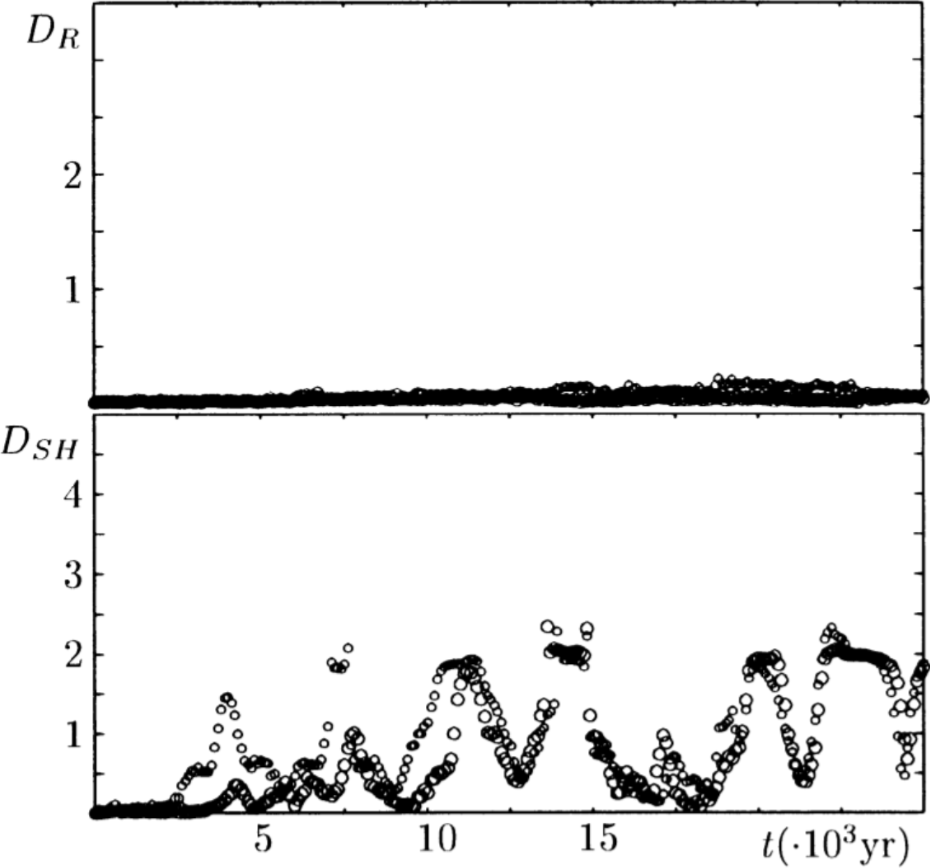
\includegraphics[width=0.5\linewidth]{img/plots/newapproach-time-evolution.png}
    \caption[Porovnání časového vývoje hodnot funkcí $D_\text{R}$ a $D_\text{SH}$]{
        Porovnání časového vývoje hodnot funkcí $D_\text{R}$ a $D_\text{SH}$\\
        {\small (zdroj: \cite{newapproach})}
    }
    \label{img:new:time}
\end{figure}

\medskip

Kompletní kritérium má předpis \cite{newapproach}
\begin{equation}
    D_\text{N}^2(A,B)=\left( U_B - U_A \right)^2 + w_1\left( \cos{\theta_B} - \cos{\theta_A} \right)^2 + \Delta\xi^2 \text{,}
\end{equation}
kde
\begin{eqnarray}
    \Delta\xi^2 &=& \min{\left\{ \left( w_2\Delta\phi_\text{I}^2 + w_3\Delta\lambda_\text{I}^2 \right),\;
                                 \left( w_2\Delta\phi_\text{II}^2 + w_3\Delta\lambda_\text{II}^2 \right) \right\}} \text{,}\\
    \Delta\phi_\text{I} &=& 2\sin{\frac{\phi_B-\phi_A}{2}} \text{,}\\
    \Delta\phi_\text{II} &=& 2\sin{\frac{180^\circ+\phi_2-\phi_1}{2}} \text{,}\\
    \Delta\lambda_\text{I} &=& 2\sin{\frac{\lambda_B-\lambda_A}{2}} \text{ a konečně}\\
    \Delta\lambda_\text{II} &=& 2\sin{\frac{180^\circ+\lambda_B-\lambda_A}{2}} \text{.}
\end{eqnarray}
$\lambda$ je zde ekliptikální délka Země v okamžiku pozorování daného meteoru a $w_2$ a $w_3$ jsou opět volitelné váhy, které se obvykle nastavují na jedničku.

Jako vhodné hranice pro kritérium $D_\text{N}$ určil \citeauthor{galligan} hodnoty \cite{galligan}
$$
    D_\text{N} \le \begin{cases}
        0{,}08 & i < 10^\circ \\
        0{,}09 & 10^\circ \le i < 90^\circ \\
        0{,}17 & i \ge 90^\circ \text{.}
    \end{cases}
$$
    \chapter{Porovnání úspěšnosti metod klasifikace}
\note{Shrnutí analýzy $D_\text{SH}$ a $D_\text{D}$ z \cite{remarks}. Experimentální(?) poznatky z \cite{galligan} a soupis vhodných rozsahů pro jednotlivé metody. Výhody $D_\text{N}$.}
    \chapter{Programový nástroj pro identifikaci meteorických rojů\label{cpt:practical}}% MARK: Praktická část

\section{Základní použití}% MARK: Základní použití
\note{Popis čtveřice režimů práce programu. Výtisk vestavěného příkazu \texttt{---help}. Příklady příkazů pro spuštění programu.}

\section{Architektura aplikace}% MARK: Architektura aplikace
\note{Popis jednotlivých modulů ve zdrojovém kódu a jejich účelů.}

\section{Technika zpracování dat}% MARK: Technika zpracování dat
\note{Vysvětlení vícevláknového zpracování. Vysvětlení prostorově stabilního řešení načítání dat a ukládání výsledků. Hledání nových meteorických rojů -- Serial Association.}

\subsection{Vícevláknové zpracování}

\subsection{Prostorová stabilita}

\subsection{Hledání nových meteorických rojů}
    \chapwithtoc{Závěr}% MARK: Závěr
V této práci jsme se seznámili s metodami primárně fotografického a video pozorování meteorů a u fotografických měření jsme důkladně prozkoumali techniku určení polohy a rychlosti meteoru z pozorování ze dvou stanic. Znalost polohy na obloze a rychlosti nám umožnila spočítat elementy dráhy meteoroidu před vstupem do zemské atmosféry.

\medskip

Elementy dráhy jsou rozhodujícím faktorem pro přiřazování meteorů do meteorických rojů. Ke zjištění, zda meteor náleží do daného meteorického roje, využíváme $D$-kritéria, jejichž princip navrhli \citeauthor{dsh}. Popsali jsme zde čtveřici těchto kritérií; od původního $D_\text{SH}$ přes modifikovaná $D_\text{D}$ a $D_\text{H}$ až po nejnovější $D_\text{N}$, které na rozdíl od předchozích kritérií pracuje s geocentrickými, nikoliv heliocentrickými, veličinami.

Na základě \citeauthor{galligan}ových simulací a vlastního testování jsme porovnali úspěšnost jednotlivých kritérií: Ze simulací vychází jako nejúspěšnější a matematicky nejlepší kritérium $D_\text{N}$, to se však při našem testování na reálných datech ukázalo jako příliš "`svolné"' v přiřazování meteorů do meteorických rojů. Unikátní přístup tohoto kritéria je ale slibný hlavně z hlediska časové stability v řádech desítek tisíc let, kde ostatní kritéria již dávno selhávají. Ukázali jsme také, že dvojice nejstarších kritérií, $D_\text{SH}$ a $D_\text{D}$, jsou naprosto obstojné, z nich odvozené $D_\text{H}$ ale bohužel i přes své vylepšené teoretické vlastnosti v praktické použitelnosti pokulhává.

\medskip

V poslední kapitole jsme na přehledové i technické úrovni popsali programový nástroj, který jsme v rámci této práce vytvořili. Jeho úkolem je zde popsaná $D$-kritéria používat k přiřazování meteorů z reálných pozorování do ustanovených meteorických rojů, či případně v reálných datech hledat nové meteorické roje.

Jedná se o program napsaný v jazyce Python, měl by tedy být své cílové skupině uživatelů, to jest fyzikům, srozumitelný. Byl navržen tak, aby co nejlépe zvládal i velké vstupní soubory s pozorováními, které se obzvláště pro hledání nových meteorických rojů dají očekávat. Jak v tomto uspěje se však ukáže až při reálném používáni, jelikož byl testován pouze na relativně malém vzorku dat, který nám byl pro jeho vývoj poskytnut.

\smallskip

Pro nás se také jednalo o první projekt v jazyce Python. I přes úvodní souboje s některými jeho vlastnostmi, jeho způsoby implementace některých v programování používaných triků a jeho silnou nevolí vůči robustní architektuře aplikace se nám ale, doufáme, podařilo vytvořit funkční, dobře vypadající a uživatelsky přívětivý program s přehledným a dobře dokumentovaným zdrojovým kódem.
% 
% Program včetně zdrojového kódu je přiložen v elektronických přílohách této práce a veřejně dostupný v repositáři \href{https://github.com/Akimayo/MeteorShowerIdentification}{github.com/Akimayo/MeteorShowerIdentification}.

    \printbibliography[title=Seznam použité literatury]
    \ask{Jak co nejvhodněji použít jména vs. iniciály? Jopek a Southworth mají jména dostupná; u Galligana, Nilssona a Hawkinse jsem bohužel ani po rozsáhlejším pátraní v publikacích a na webech univerzit nenašel.}

    \noindent
    \note{\textbf{Statistics of Meteor Streams} \cite{dsh}: míra orbitální odlišnosti $D(A,B)$, odlišnost od průměru $D(M,N)$, zanedbatelnost $\nu$, závislost orbitálních proměnných, odhad náhodných přiřazení orbitů do rojů, klasifikace rojů (major/minor/spurious), tabulky orbitálních parametrů, náležitost rojů ke kometám, perturbace}\\
    \note{\textbf{A Southern Hemisphere Radio Survey...} \cite{radiosurvey}: technika měření, podmínky seskupování orbitů do rojů, vyřazení malých skupin, podobnost ``minor'' a ``major'' rojů, dvojí detekce rojů s nízkou inklinací}\\
    \note{\textbf{Remarks...} \cite{remarks}: příklad fiktivních orbitů protínající oběžnou dráhu Země, úměrnost $D_{SH}$ rychlosti, Drummondova funkce odlišnosti, nežádoucí jevy $D_{SH}$ a $D_D$, rozbor oblouků vs. tětiv ve vzorcích, hybridní funkce odlišnosti $D_H$}\\
    \note{\textbf{...a new approach} \cite{newapproach}: Keplerovské souřadnice, lineární závislost Keplerovských souřadnic v $D_{SH}$, geocentrický přístup, semi-invariantní veličiny, geocentrická funkce odlišnosti $D_N$}\\
    \note{\textbf{Performance of the $D$-criteria...} \cite{galligan}: hranice hodnot odlišnosti pro různé inklinace, sporadické pozadí, porovnání účinnosti metod}\\
    \note{\textbf{...Comet and Meteor Shower Association} \cite{cometassoc}: příslušnost některých meteorických rojů kometám, tabulka elementů dráhy těchto komet, poznámky k $D_\text{SH}$, lepší rozpis $D_\text{D}$}\\
    \note{\textbf{...Photographic Fireball Networks} \cite{ceplecha}: metody fotografického záznamu meteoritů, definice radiantu, výpočet orbitu, Gaussova gravitační konstanta $k=0{,}01720209895$}\\
    \note{\textbf{Definitions...in meteor astronomy} \cite{meteorastro}: definice pojmů meteorit, meteoroid a meteor}\\

    \noindent
    \ask{DRUMMOND, J. D. 1979. On the meteor/comet orbital discriminant D. \textit{Proc. Southwest Reg. Conf. Aslron. Astrophys.} \textbf{5, 83-86}.}

    \listoffigures
    \listoftables
\end{document}